\chapter{METODOLOGI}
\label{chap:metodologi}

Rancangan implementasi \emph{multi-tenancy} untuk \emph{provisioning}
klaster Kubernetes dimulai dari membuat aplikasi \emph{service} untuk \emph{provisioning}
yang terletak di komputer \emph{worker} untuk membuat
\emph{virtual machine}, kemudian membuat situs web \emph{dashboard} yang nantinya
digunakan oleh \emph{user} untuk membuat klaster Kubernetes secara dinamis dan sewaktu-waktu
menggunakan \emph{virtual machine} yang dibuat oleh aplikasi \emph{provisioning}.
Rancangan tahapan penyelesain implementasi tugas akhir ini
dapat dilihat pada gambar \ref{fig:top-level-implementation}.

\begin{figure}[H]
  \centering
  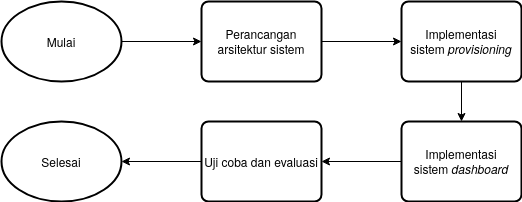
\includegraphics[scale=0.6]{gambar/top-level-implementation.png}
  \caption{Rancangan Penyelesaian Implementasi Tugas Akhir}
  \label{fig:top-level-implementation}
\end{figure}

Berdasarkan gambar \ref{fig:top-level-implementation} di atas, tahapan pertama
dalam rancangan implementasi tugas akhir adalah perancangan arsitektur sistem.
Tahapan perancangan arsitektur sistem berdasarkan kebutuhan sistem yang diperlukan
yaitu situs web sebagai \emph{dashboard} dan aplikasi \emph{provisioning}
untuk membuat \emph{virtual machine}. Setelah perancangan arsitektur sistem telah
selesai, implementasi dari rancangan sebelumnya akan dilakukan. Tahap terakhir
dari tugas akhir ini adalah uji coba dan evaluasi dari sistem yang telah dirancang.
Uji coba dan evaluasi ini bertujuan untuk memeriksa apakah sistem yang telah
diimplementasikan dapat berjalan sesuai kebutuhan dari tugas akhir ini.

\section{Perancangan Arsitektur Sistem}
\label{sec:perancanganarsitektursistem}

Secara garis besar, \emph{workflow} dari implementasi tugas akhir ini dapat dilihat
pada gambar \ref{fig:website-flowchart}. Selain itu, gambaran dari arsitektur sistem
implementasi tugas akhir ini terdapat
pada gambar \ref{fig:server-worker-top-level}. Berdasarkan gambar \ref{fig:server-worker-top-level},
komunikasi antara \emph{worker} dan server utama adalah komunikasi dua arah. Server utama
berkomunikasi dengan \emph{worker} untuk membuat \emph{virtual machine} dan \emph{worker}
berkomunikasi dengan server utama untuk memberi status bahwa \emph{worker} sudah siap
dalam menerima permintaan untuk membuat \emph{virtual machine} serta memberi status dari
pembuatan \emph{virtual machine}.

Setiap komputer fisik yang akan dijadikan \emph{worker} memerlukan aplikasi
atau sebuah \emph{service} yang dapat menerima permintaan pembuatan 
\emph{virtual machine} yang dikirimkan melalui server utama. Selain itu,
server utama juga memerlukan aplikasi yang dapat digunakan oleh pengguna
untuk membuat klaster dengan \emph{virtual machine} pada \emph{worker}.

\begin{figure}[H]
  \centering
  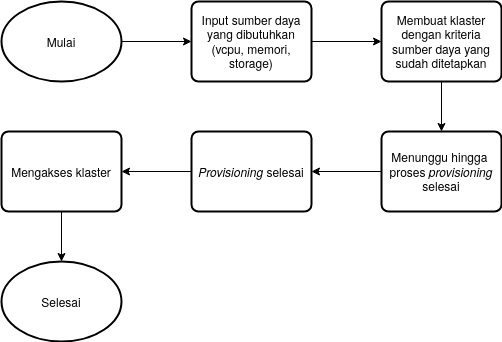
\includegraphics[scale=0.6]{gambar/flowchart-website.png}
  \caption{\emph{Workflow} Penggunaan Aplikasi}
  \label{fig:website-flowchart}
\end{figure}

\begin{figure}[H]
  \centering
  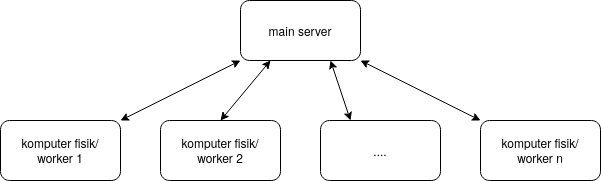
\includegraphics[scale=0.6]{gambar/server-worker-top-level.png}
  \caption{Gambaran Arsitektur Sistem}
  \label{fig:server-worker-top-level}
\end{figure}

\section{Implementasi Sistem \emph{Provisioning}}
\label{sec:implementasi-sistem-provisioning}

Sistem \emph{provisioning} pada setiap komputer \emph{worker} secara fungsi dapat dipisah
menjadi dua bagian besar, yaitu bagian server untuk menerimaa permintaan pembuatan klaster yang dikirim
oleh server utama dan bagian pembuatan \emph{virtual machine}.

\subsection{Implementasi Server}
\label{sec:server}

Komputer \emph{worker} menerima \emph{request} pembuatan klaster melalui jaringan internet.
Oleh karena itu, \emph{worker} dapat menerima \emph{request} dengan membuka dan mendengarkan \emph{port}
untuk menerima \emph{request} dari server utama. Implementasi tugas akhir ini menggunakan protokol
RPC dengan gRPC untuk menerima \emph{request} tersebut.

\begin{lstlisting}[
  caption={Definisi Prosedur RPC pada Komputer \emph{Worker}},
  label={lst:rpc-procedure}
]
syntax = "proto3";

option go_package = "./services/model/proto-model";

enum Status {
  STATUS_UNSPECIFIED = 0;
  STATUS_AVAILABLE = 1;
  STATUS_UNAVAILABLE = 2;
}

message Empty {}

message CreateNodeRequirements {
  int64 cpu = 1;
  int64 memory = 2;
  int64 storage = 3;
}

// create master
message CreateMasterRequest {
  string token = 1;
  CreateNodeRequirements requirements = 2;
}

message CreateMasterResponse {
  string ip_address = 1;
}

// create worker
message CreateWorkerRequest {
  string token = 1;
  string ip_address = 2;
  CreateNodeRequirements requirements = 3;
}

message CreateWorkerResponse {}

service NodeService {
  rpc CreateMaster(CreateMasterRequest) returns (CreateMasterResponse) {}
  rpc CreateWorker(CreateWorkerRequest) returns (CreateWorkerResponse) {}
}
\end{lstlisting}

Kode sumber \ref{lst:rpc-procedure} menunjukkan fungsi atau prosedur
yang disediakan oleh \emph{worker} menggunakan protokol RPC. Untuk membuat prosedur
di gRPC, format yang dipakai adalah format Protobuf. Protobuf merupakan format
yang digunakan oleh gRPC sebagai \emph{Interface Definition Language}.

Prosedur yang sudah ditulis menggunakan Protobuf akan dikonversi
ke bahasa pemrograman yang diinginkan. Hasil konversi tersebut hanya
berupa fungsi atau prosedur tanpa isi. Isi atau \emph{logic} dari fungsi atau prosedur
tersebut harus dibuat sesuai dengan keinginan pengguna. Hasil konversi dari Protobuf
dapat dibagikan ke komputer lainnya yang memerlukan prosedur tersebut. 

Pada implementasi tugas akhir ini, komputer \emph{worker} menerima
hasil konversi dari prosedur dari Protobuf dan membuat isi dari
prosedur yang sudah ditetapkan. Server utama juga menerima hasil konversi
dan akan menggunakannya untuk menjalankan fungsi atau prosedur tersebut di komputer
\emph{worker}. Isi dari prosedur yang akan dijalankan di komputer \emph{worker} terdapat
pada kode sumber \ref{lst:isi-prosedur}. Isi prosedur tersebut adalah \emph{logic}
untuk membuat \emph{virtual machine} yang berjenis \emph{master node} atau \emph{worker node}.
Perbedaan dari keduanya adalah \emph{master node} akan bertugas menjadi \emph{control plane}
dari klaster Kubernetes yang dibuat nantinya.

\clearpage

\lstinputlisting[
  language=Go,
  caption={Isi Prosedur pada Komputer \emph{Worker}},
  label={lst:isi-prosedur}
]{program/rpc-procedure-logic.go}

Komputer \emph{worker} perlu mendengarkan \emph{request} pembuatan melalui
protokol gRPC yang sudah ditetapkan sebelumnya. \emph{Library} gRPC pada Golang
menyediakan API untuk server untuk mendengarkan \emph{request} gRPC di \emph{port}
tertentu. Setelah server mendengarkan di \emph{port} yang telah ditentukan, maka
server tersebut dapat menerima \emph{request} RPC dengan prosedur atau fungsi
yang sudah dibuat melalui \emph{stub}. Kode sumber untuk menjalankan
gRPC server dapat dilihat pada kode sumber \ref{lst:rpc-server-start}.

\lstinputlisting[
  language=Go,
  caption={Memulai gRPC Server},
  label={lst:rpc-server-start},
  style=codestyle,
]{program/rpc-start-server.go}

\subsection{Implementasi \emph{Provisioning}}
\label{sec:provisioning}

Setelah komputer menerima \emph{request} pembuatan klaster melalui RPC,
\emph{request} tersebut diteruskan ke bagian \emph{provisioning}. Alur 
implementasi \emph{provisioning} dari implementasi ini adalah mempersiapkan
sistem operasi Linux yang akan digunakan sebagai sistem operasi dari
\emph{virtual machine}, mempersiapkan Linux \emph{bridge},
implementasi QEMU dan Libvirt untuk membuat \emph{virtual machine},
implementasi Cloud-init untuk mengkustomisasi \emph{virtual machine}, 
serta implementasi \emph{queue} dan \emph{worker}.
% dan implementasi Websocket untuk \emph{logging}.

\subsubsection{Persiapan Linux untuk \emph{Virtual Machine}}
\label{sec:persiapan-linux-untuk-virtual-machine}

Dalam mempersiapkan sistem operasi Linux yang akan dipakai, terdapat beberapa
hal yang harus dipertimbangkan. Karena \emph{virtual machine} yang akan digunakan
harus siap dengan konfigurasi Cloud-init, maka Linux yang digunakan bukan Linux
yang berbentuk ISO. Linux berbentuk ISO pada saat \emph{booting} akan mengarahkan
\emph{user} untuk proses instalasi sistem operasi Linux dan proses tersebut memerlukan
interaksi dengan pengguna. Selain itu, Linux dalam bentuk ISO tidak memiliki Cloud-init
sehingga tidak memungkinkan untuk menjalankan proses Cloud-init.

Untuk memenuhi kebutuhan tersebut, maka \emph{image} Linux yang digunakan
adalah \emph{image} yang khusus untuk kebutuhan \emph{cloud}. Ubuntu merupakan
salah satu distribusi Linux yang menyediakan \emph{image} khusus tersebut.
Pada implementasi tugas akhir ini, versi Ubuntu yang digunakan adalah Ubuntu 24.10
dengan nama kode "Oracular Oriole". Jenis \emph{file} dari \emph{image} yang akan digunakan
adalah \emph{file} dengan ekstensi .img yang merupakan format \emph{file} untuk \emph{disk image}
yang digunakan oleh QEMU.

Versi Ubuntu yang digunakan pada \emph{cloud image} adalah versi Ubuntu Server yang
berukuran lebih kecil dari \emph{desktop image} dan berisi aplikasi dan \emph{tools}
yang sering digunakan pada server. Namun pada Ubuntu \emph{cloud image}, tidak ada
kata sandi untuk bisa \emph{login} ke \emph{root} pada sistem operasi. Untuk bisa \emph{login},
dibutuhkan kata sandi untuk \emph{root} pada \emph{cloud image} tersebut. Salah satu \emph{tool} yang
dapat digunakan untuk memodifikasi kata sandi dari \emph{user} pada file .img adalah \emph{virt-customize}.
Untuk menambahkan kata sandi untuk \emph{root} menggunakan \emph{virt-customize} adalah
sebagai berikut:

\begin{lstlisting}[
  style=clistyle,
  caption={\emph{Command} Linux untuk Konfigurasi \emph{Cloud Image}}
]
# virt-customize --add oracular-server-cloudimg-amd64.img --root-password password:root
\end{lstlisting}

Pada \emph{command} di atas, \lstinline{oracular-server-cloudimg-amd64.img} menandakan \emph{file disk image}
mana yang ingin dimodifikasi, \lstinline{--root-password password:root} menandakan bahwa kata sandi
dari \emph{user root} adalah root.

Setelah \emph{user root} sudah memiliki kata sandi, \emph{user root} dapat digunakan
pada Ubuntu tersebut. Pada implementasi tugas akhir ini, modifikasi lain yang dilakukan
terhadap \emph{cloud image} ini adalah mengunduh \emph{binary} dari K3s dan Helm untuk mengurangi
waktu yang dibutuhkan untuk membuat \emph{virtual machine}. Pada implementasi tugas akhir ini,
versi K3s yang digunakan adalah v1.33.1+k3s1 (99d91538) dan versi Helm yang digunakan adalah
v3.18.1 dengan \emph{commit} terakhir f6f87.

\begin{figure}[H]
  \centering
  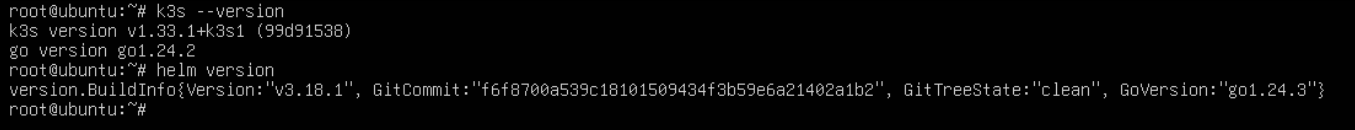
\includegraphics[scale=0.4]{gambar/k3s-helm-version.png}
  \caption{Versi K3s dan Helm}
  \label{fig:k3s-helm-version}
\end{figure}

\emph{Cloud image} Ubuntu secara \emph{default} sudah memiliki Cloud-init. Cloud-init tersebut
tidak perlu dikonfigurasi untuk dapat digunakan. Pada saat \emph{booting virtual machine} untuk yang
pertama kali dengan menggunakan \emph{file} konfigurasi yang diperlukan, Cloud-init akan secara otomatis
menjalankan konfigurasi dari \emph{file} tersebut.

\subsubsection{Persiapan Linux \emph{Bridge}}
\label{sec:persiapan-linux-bridge}

Proses penggabungan \emph{worker node} menggunakan K3s memerlukan alamat IP
dari \emph{control plane}. Karena \emph{virtual machine} yang bertugas menjadi
\emph{worker node} tidak selalu berada di komputer fisik yang sama, sehingga
\emph{control plane} dan \emph{worker node} memerlukan alamat IP di jangkauan
yang sama dengan komputer \emph{host} agar dapat berkomunikasi satu sama lain.
\emph{Virtual machine} dapat memiliki alamat IP di jangkauan yang sama dengan
alamat IP dari \emph{host} menggunakan Linux \emph{bridge}.

Untuk membuat Linux \emph{bridge} di sistem operasi Linux pada implementasi tugas akhir ini,
\emph{tools} NetworkManager akan digunakan. Pemilihan \emph{tools} tersebut karena
NetworkManager merupakan \emph{default tools} yang digunakan pada distribusi Linux
Ubuntu. Selain itu, NetworkManager juga dapat mengatur koneksi internet pada
komputer, termasuk pembuatan Linux \emph{bridge}. Untuk membuat Linux \emph{bridge}
yang bernama k3s-br0 dan \emph{network interface} dari ethernet yang digunakan
adalah enp1s0, dapat menggunakan \emph{command line} sebagai berikut:

\begin{lstlisting}[
  style=clistyle,
  caption={\emph{Command} Linux untuk Konfigurasi Linux \emph{Bridge}},
]
# nmcli con add type bridge ifname k3s-br0 con-name k3s-br0
# nmcli con add type bridge-slave ifname enp1s0 master k3s-br0
# nmcli con down enp1s0
# nmcli con up k3s-br0
\end{lstlisting}

Setelah itu, komputer akan tetap tersambung dengan koneksi internet melalui
\emph{network interface} enp1s0 dan Linux \emph{bridge} k3s-br0 juga aktif.
Linux \emph{bridge} k3s-br0 akan digunakan pada saat membuat \emph{virtual machine}.
\subsubsection{Implementasi Cloud-init}
\label{sec:implementasi-cloud-init}

Konfigurasi Cloud-init yang digunakan untuk \emph{virtual machine} yang bertugas sebagai \emph{control plane}
dan \emph{worker node} berbeda. Untuk \emph{virtual machine} yang bertugas menjadi \emph{control plane},
ada konfigurasi tambahan dibandingkan dengan \emph{virtual machine} yang bertugas menjadi \emph{worker node}.

\emph{Control plane} dan \emph{worker node} menggunakan konfigurasi jaringan yang sama. \emph{Cloud image}
dari Ubuntu menggunakan \emph{network interface} enp1s0 sebagai \emph{network interface} untuk
koneksi dengan ethernet. Oleh karena itu, \emph{control plane} dan \emph{worker node} menggunakan
konfigurasi jaringan yang sama karena menggunakan \emph{cloud image} yang sama. Kode sumber untuk
konfigurasi jaringan melalui Cloud-init terdapat pada kode sumber \ref{lst:konfigurasi-jaringan}.

\lstinputlisting[
  caption={Konfigurasi Jaringan},
  label={lst:konfigurasi-jaringan},
  style=codestyle,
]{program/cloud-init-network-configuration.yaml}

Pada kode sumber \ref{lst:konfigurasi-jaringan}, sintaks konfigurasi yang dipakai adalah sintaks
konfigurasi versi 2 dari Cloud-init. \emph{Network interface} yang dikonfigurasi adalah \emph{network interface}
enp1s0. \emph{Network interface} tersebut merupakan \emph{default network interface} yang digunakan
oleh \emph{cloud image} Ubuntu untuk jaringan ethernet. Protokol dhcp digunakan agar \emph{virtual machine} mendapatkan
IP secara dinamis dari \emph{host} yang menyediakan Linux \emph{bridge}.

Setelah melakukan konfigurasi jaringan, akan dilakukan konfigurasi lainnya.
Pada \emph{control plane}, konfigurasi lanjutan dari Cloud-init dapat dilihat 
pada kode sumber \ref{lst:konfigurasi-lanjutan-control-plane}.
Untuk \emph{worker node}, konfigurasi lanjutan dari Cloud-init dapat dilihat
pada kode sumber

\lstinputlisting[
  caption={Konfigurasi Lanjutan pada \emph{Control Plane}},
  label={lst:konfigurasi-lanjutan-control-plane},
  style=codestyle,
]{program/cloud-init-control-plane-configuration.yaml}

Kode sumber \ref{lst:konfigurasi-lanjutan-control-plane}
mengkonfigurasi beberapa hal pada \emph{control plane} seperti berikut:

\begin{enumerate}
  
  \item \lstinline{hostname} menentukan nama \emph{hostname} pada \emph{virtual machine}.
    Konfigurasi Cloud-init akan digunakan pada bahasa Golang sehingga \lstinline{%s}
    akan dipakai karena penentuan nama \emph{hostname} dilakukan secara dinamis.

  \item \lstinline{locale} menentukan \emph{locale} yang akan dipakai.

  \item \lstinline{timezone} menentukan waktu yang dipakai yaitu Waktu Indonesia Barat (WIB)

  \item \lstinline{users} menandakan konfigurasi \emph{user} yang akan digunakan. Pada
    contoh tersebut, terdapat dua \emph{user} yang akan dibuat pada \emph{virtual machine},
    yaitu \emph{user default} dan \emph{user} dengan nama user. \emph{User default} merupakan
    \emph{user} admin bawaan.

  \item \lstinline{write_files} berisi \emph{file} apa saja yang akan dibuat beserta konten
    dari \emph{file} tersebut. Pada contoh kode sumber, terdapat 3 \emph{file} yang akan dituliskan.
    \emph{File} pertama adalah \emph{file} berekstensi yaml yang akan digunakan untuk membuat
    ServiceAccount pada klaster Kubernetes. \emph{File} selanjutnya adalah \emph{file} berekstensi
    yaml yang akan digunakan untuk RoleBinding ke ServiceAccount yang dibuat menggunakan
    \emph{file} pertama. \emph{File} terakhir merupakan \emph{file} konfigurasi 
    \emph{service} systemd untuk \emph{dashboard} Kubernetes.

  \item \lstinline{runcmd} merupakan daftar dari \emph{command line} yang akan dijalankan.
    \emph{Command line} yang akan dijalankan adalah \emph{command line} untuk membuat klaster
    Kubernetes menggunakan K3s, menambahkan Repository Helm kubernetes-dashboard ke dalam
    klaster Kubernetes, menggunakan \emph{file} untuk klaster Kubernetes yang sudah dibuat
    melalui \lstinline{write_files}, serta menjalankan \emph{service} systemd untuk
    kubernetes-dashboard.

\end{enumerate}

\lstinputlisting[
  caption={Konfigurasi Lanjutan pada \emph{Worker Node}},
  label={lst:konfigurasi-lanjutan-worker-node},
  style=codestyle,
]{program/cloud-init-worker-node-configuration.yaml}

Kode sumber \ref{lst:konfigurasi-lanjutan-worker-node}
mengkonfigurasi beberapa hal pada \emph{worker node} seperti berikut:

\begin{enumerate}
  
  \item \lstinline{hostname} menentukan nama \emph{hostname} pada \emph{virtual machine}.
    Konfigurasi Cloud-init akan digunakan pada bahasa Golang sehingga \lstinline{%s}
    akan dipakai karena penentuan nama \emph{hostname} dilakukan secara dinamis.

  \item \lstinline{locale} menentukan \emph{locale} yang akan dipakai.

  \item \lstinline{timezone} menentukan waktu yang dipakai yaitu Waktu Indonesia Barat (WIB)

  \item \lstinline{users} menandakan konfigurasi \emph{user} yang akan digunakan. Pada
    contoh tersebut, terdapat dua \emph{user} yang akan dibuat pada \emph{virtual machine},
    yaitu \emph{user default} dan \emph{user} dengan nama user. \emph{User default} merupakan
    \emph{user} admin bawaan.

  \item \lstinline{runcmd} merupakan daftar dari \emph{command line} yang akan dijalankan.
    \emph{Command line} yang akan dijalankan adalah \emph{command line} untuk bergabung ke
    klaster Kubernetes yang dibuat oleh \emph{control plane} menggunakan K3s.

\end{enumerate}

\subsubsection{Implementasi \emph{Queue} dan \emph{Worker}}
\label{sec:implementasi-queue-dan-worker}

Mekanisme \emph{queue} akan digunakan pada saat proses \emph{provisioning}
\emph{virtual machine} untuk menghindari permasalahan yang dapat muncul ketika
lebih dari satu \emph{virtual machine} dibuat secara bersamaan. \emph{Queue}
akan berisi permintaan serta parameter yang dibutuhkan untuk membuat
\emph{virtual machine}. Untuk mengerjakan permintaan tersebut, sistem \emph{worker}
akan digunakan.

Redis akan digunakan dalam mengimplementasikan mekanisme \emph{queue}. Redis mendukung
penggunaan basis data dalam bentuk \emph{queue} yang bersifat \emph{First In First Out}.
Pada struktur data \emph{queue}, dua operasi utama yang dibutuhkan adalah penambahan data
ke \emph{queue} dan pengambilan data dari \emph{queue}. Kode sumber penambahan data \emph{queue}
dan pengambilan data dari \emph{queue} dapat dilihat pada kode sumber
\ref{lst:penambahan-data-ke-queue} dan \ref{lst:pengambilan-data-dari-queue}.

\lstinputlisting[
  language=go,
  caption={Operasi Penambahan Data ke \emph{Queue}},
  label={lst:penambahan-data-ke-queue},
  style=codestyle,
]{program/redis-add-to-queue.go}

\lstinputlisting[
  language=go,
  caption={Operasi Pengambilan Data dari \emph{Queue}},
  label={lst:pengambilan-data-dari-queue},
  style=codestyle,
]{program/redis-queue-pop.go}

Selain itu, Redis juga dapat digunakan sebagai implementasi dari paradigma \emph{message delivery}
dalam bentuk \emph{publisher} dan \emph{subscriber}. Subjek yang menjadi
\emph{subscribe} dapat menunggu pesan dalam sebuah \emph{channel} dan 
\emph{publisher} dapat mengirim pesan ke dalam \emph{channel} tersebut.
Pada implementasi tugas akhir ini, \emph{message delivery} digunakan
sebagai bentuk komunikasi antara \emph{worker} dengan sistem \emph{provisioning}.
Sistem komunikasi tersebut bertujuan agar \emph{worker} dapat menerima hasil
dari \emph{provisioning}. Kode sumber fungsi \emph{publisher} dan \emph{subscriber}
pada \emph{queue} dapat dilihat pada kode sumber \ref{lst:queue-pub-sub}.

\lstinputlisting[
  language=go,
  caption={Operasi \emph{Publisher} dan \emph{Subscriber}},
  label={lst:queue-pub-sub},
  style=codestyle,
]{program/redis-queue-pub-sub.go}

\emph{Worker} digunakan untuk menjalankan tugas \emph{provisioning}
yang terdapat pada \emph{queue}. \emph{Worker} akan diimplementasikan
sebagai sebuah goroutine menggunakan bahasa pemrograman Golang. Goroutine merupakan
fitur pada bahasa pemrograman untuk menjalankan sebuah fungsi atau proses
di \emph{background} sehingga tidak terjadi situasi \emph{blocking}. Kode sumber
fungsi \emph{worker} dapat dilihat pada kode sumber \ref{lst:fungsi-worker}.

\clearpage

\lstinputlisting[
  language=go,
  caption={Fungsi pada \emph{Worker}},
  label={lst:fungsi-worker},
  style=codestyle,
]{program/worker.go}

Pada kode sumber \ref{lst:fungsi-worker}, \emph{worker} memanggil fungsi
dari \emph{queue} yaitu fungsi untuk mengambil data dari \emph{queue}
di dalam sebuah \emph{loop} yang tidak akan pernah selesai. Setelah
mendapatkan data permintaan dan parameter yang dibutuhkan untuk \emph{provisioning},
permintaan dan parameter diteruskan ke fungsi untuk membuat \emph{instance}
dari \emph{virtual machine}.

% \subsubsection{Implementasi Websocket}
% \label{sec:implementasi-websocket}
%
% Untuk menunjukkan proses dalam pembuatan \emph{virtual machine}

\subsubsection{Implementasi QEMU dan Libvirt}
\label{sec:implementasi-libvirt}

Libvirt menyediakan \emph{bindings} untuk banyak bahasa pemrograman
untuk berkomunikasi dengan Libvirt. Libvirt juga menyediakan API untuk
mengelola \emph{virtual machine} dan teknologi virtualisasi.

Dalam implementasi tugas akhir ini, QEMU dan Libvirt akan digunakan.
Untuk menggunakan QEMU sebagai emulator dan interaksi dengan QEMU menggunakan Libvirt,
Libvirt memerlukan konfigurasi koneksi dengan QEMU. Kode sumber untuk konfigurasi
tersebut dapat dilihat pada kode sumber \ref{lst:konfigurasi-qemu-libvirt}.

\lstinputlisting[
  language=go,
  caption={Konfigurasi QEMU dengan Libvirt},
  label={lst:konfigurasi-qemu-libvirt},
  style=codestyle,
]{program/libvirt-connection.go}

Pada kode sumber \ref{lst:konfigurasi-qemu-libvirt}, \lstinline{qemu:///system} akan
digunakan sebagai koneksi ke \emph{daemon} dari Libvirt yang berjalan sebagai \emph{root}.
Koneksi tersebut akan digunakan untuk komunikasi antara \emph{bindings} dari Libvirt yang
dipakai dengan teknologi virtualisasi QEMU.

Proses \emph{provisioning} menggunakan Libvirt terdiri dari beberapa langkah, yaitu:

\begin{enumerate}

  \item Membuat \emph{file} konfigurasi untuk Cloud-init

    Untuk menggunakan Cloud-init dengan konfigurasi yang diinginkan, \emph{file}
    yang berisi konfigurasi Cloud-init harus diubah menjadi \emph{disk} dan digunakan
    pada saat membuat \emph{virtual machine}. Kode sumber untuk membuat \emph{file}
    konfigurasi jaringan terdapat pada kode sumber \ref{lst:pembuatan-file-konfigurasi-jaringan}.

    \lstinputlisting[
      language=go,
      caption={Pembuatan \emph{File} Konfigurasi Jaringan},
      label={lst:pembuatan-file-konfigurasi-jaringan},
      style=codestyle,
    ]{program/network-and-others-cloud-init.go}

    Setelah \emph{file} konfigurasi jaringan telah dibuat, \emph{file}
    konfigurasi lanjutan untuk Cloud-init akan dibuat. Kode sumber untuk membuat
    \emph{file} konfigurasi lanjutan \emph{virtual machine} yang bertugas
    menjadi \emph{control plane} dan \emph{worker node} terdapat pada kode sumber
    \ref{lst:pembuatan-file-konfigurasi-control-plane} dan \ref{lst:pembuatan-file-konfigurasi-worker-node}.

    \lstinputlisting[
      language=go,
      caption={Pembuatan \emph{File} Konfigurasi Lanjutan \emph{Control Plane}},
      label={lst:pembuatan-file-konfigurasi-control-plane},
      style=codestyle,
    ]{program/control-plane-cloud-init.go}

    \lstinputlisting[
      language=go,
      caption={Pembuatan \emph{File} Konfigurasi Lanjutan \emph{Worker Node}},
      label={lst:pembuatan-file-konfigurasi-worker-node},
      style=codestyle,
    ]{program/worker-node-cloud-init.go}

    Pada kode sumber \ref{lst:pembuatan-file-konfigurasi-control-plane}
    dan \ref{lst:pembuatan-file-konfigurasi-worker-node}, \emph{disk}
    dibuat menggunakan \emph{tool} \lstinline{cloud-localds}. \emph{Tool}
    tersebut menghasilkan \emph{file} berekstensi iso yang nantinya akan
    dipasangkan ke \emph{virtual machine}.

  \item Menyalin \emph{cloud image}

    \emph{Cloud image} yang sudah dimodifikasi sebelumnya disalin untuk
    setiap \emph{virtual machine} yang akan dibuat dan dilakukan proses
    \emph{resize} sesuai dengan ukuran penyimpanan yang diinginkan oleh
    pengguna. Kode sumber untuk menyalin dan melakukan proses \emph{resize}
    terdapat pada kode sumber \ref{lst:penyalinan-cloud-image}

    \lstinputlisting[
      language=go,
      caption={Penyalinan \emph{cloud image}},
      label={lst:penyalinan-cloud-image},
      style=codestyle,
    ]{program/image-copy-and-resize.go}

  \item Membuat \emph{virtual machine}

    Untuk membuat \emph{virtual machine} melalui Libvirt, konfigurasi
    mengenai \emph{virtual machine} tersebut perlu diberikan. Libvirt menggunakan
    \emph{file} berekstensi xml untuk konfigurasi \emph{virtual machine}.
    Kode sumber untuk mengatur konfigurasi xml \emph{virtual machine} terdapat
    pada kode sumber \ref{lst:konfigurasi-xml-virtual-machine}

    \lstinputlisting[
      language=go,
      caption={Konfigurasi xml \emph{Virtual Machine}},
      label={lst:konfigurasi-xml-virtual-machine},
      style=codestyle,
    ]{program/libvirt-xml-base.go}

    Setelah konfigurasi xml dari \emph{virtual machine} telah dibuat, Libvirt
    dapat menggunakan konfigurasi tersebut untuk membuat \emph{virtual machine}.
    Kode sumber untuk membuat \emph{virtual machine} menggunakan konfigurasi
    xml dapat dilihat pada kode sumber \ref{lst:pembuatan-vm-dengan-xml}.

    \lstinputlisting[
      language=go,
      caption={Pembuatan \emph{Virtual Machine} dengan Konfigurasi xml},
      label={lst:pembuatan-vm-dengan-xml},
      style=codestyle,
    ]{program/libvirt-full.go}

  \item Menunggu proses Cloud-init

    Cloud-init memerlukan beberapa waktu untuk menyelesaikan tugasnya.
    Beberapa proses memerlukan proses yang dijalankan oleh Cloud-init
    untuk selesai terlebih dahulu. Untuk menunggu proses Cloud-init selesai,
    ditunjukkan pada kode sumber \ref{lst:menunggu-cloud-init}.

    \lstinputlisting[
      language=go,
      caption={Menunggu Proses Cloud-init Selesai},
      label={lst:menunggu-cloud-init},
      style=codestyle,
    ]{program/wait-cloud-init.go}

    Pada kode sumber \ref{lst:menunggu-cloud-init}, fungsi \lstinline{guestAgentExecStatus}
    dipanggil. Fungsi tersebut digunakan untuk menjalankan \emph{command line interface}
    pada \emph{virtual machine} dengan mengutilisasi qemu-guest-agent. Untuk mengetahui
    status dari Cloud-init pada \emph{virtual machine} tersebut, Cloud-init menyiapkan
    \emph{command line interface} yang dapat digunakan untuk mengetahui dan menunggu proses
    dari Cloud-init. Fungsi \lstinline{guestAgentExecStatus} dapat dilihat pada \ref{lst:fungsi-untuk-menjalankan-cli}.

    \lstinputlisting[
      language=go,
      caption={Fungsi untuk Menjalankan \emph{Command Line Interface} pada \emph{Virtual Machine}},
      label={lst:fungsi-untuk-menjalankan-cli},
      style=codestyle,
    ]{program/guest-agent-exec.go}

\end{enumerate}

\section{Implementasi Situs Web}
\label{sec:implementas-situs-web}

Situs web yang dibuat akan digunakan sebagai pengguna untuk membuat
klaster Kubernetes menggunakan \emph{virtual machine} yang dibuat
oleh sistem \emph{provisioning}. Implementasi situs web dibagi menjadi
dua yaitu implementasi bagian \emph{frontend} dan bagian \emph{backend}.

\subsection{Implementasi \emph{Frontend}}
\label{subsec:implementas-frontend}

Situs web \emph{dashboard} merupakan antarmuka yang akan digunakan oleh \emph{user}
untuk membuat klaster Kubernetes. Pada situs web tersebut, terdapat
informasi mengenai identitas komputer yang siap
menerima permintaan untuk membuat \emph{virtual machine}.
Tampilan dari \emph{dashboard} dapat dilihat pada gambar
dan \ref{fig:dashboard-with-node}.

\begin{figure}[H]
  \centering
  \fbox{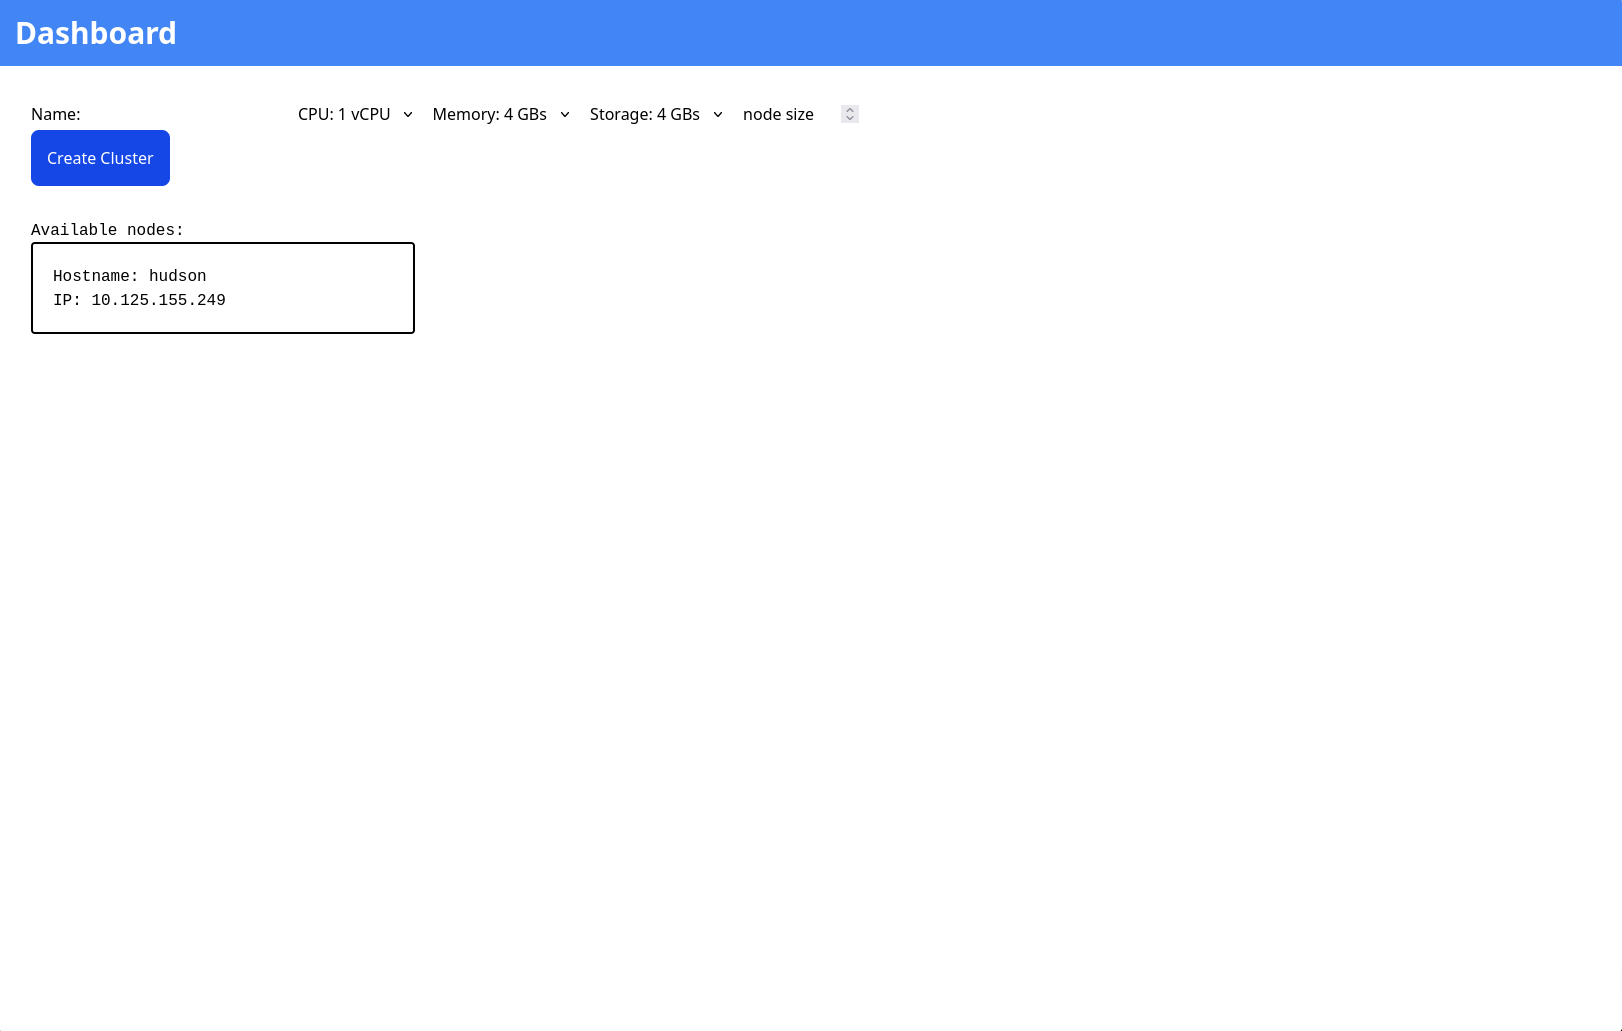
\includegraphics[scale=0.35]{gambar/dashboard-with-node.png}}
  \caption{Tampilan \emph{Dashboard}}
  \label{fig:dashboard-with-node}
\end{figure}

Pada contoh gambar \ref{fig:dashboard-with-node}, terdapat satu komputer \emph{worker}
yang siap untuk menerima permintaan, yaitu komputer yang memiliki \emph{hostname} hudson dan alamat
ip 10.125.155.249.

% TODO: implementasi backend
\subsection{Implementasi \emph{Backend}}
\label{subsec:implementas-backend}

Bagian \emph{backend} dari situs web bertanggung jawab untuk menangani permintaan
yang dibuat pengguna pada bagian \emph{frontend}. Selain itu, bagian \emph{backend}
juga bertanggung jawab untuk melakukan komunikasi dengan komputer \emph{worker} menggunakan
protokol RPC melalui gRPC. Garis besar pertukaran informasi dan komunikasi
dapat dilihat pada gambar \ref{fig:frontend-backend-worker}.

\begin{figure}[H]
  \centering
  \fbox{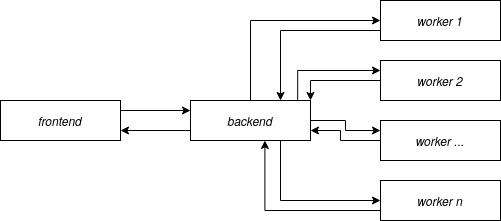
\includegraphics[scale=0.55]{gambar/frontend-backend-worker.png}}
  \caption{Komunikasi \emph{Frontend-Backend-Worker}}
  \label{fig:frontend-backend-worker}
\end{figure}
